\section{Estado del arte}

En esta sección, el objetivo es analizar la literatura reciente y los artículos publicados sobre el entrenamiento de modelos de aprendizaje profundo, tanto a través de técnicas basadas en GD como MH. Para un mejor contexto, realizaremos una búsqueda en la base de datos de referencias bibliográficas y citas Scopus\footnote{\url{https://www.scopus.com/}}, con el fin de conocer el estado actual de la literatura. 



Vamos a realizar una búsqueda en el ámbito del entrenamiento de modelos de aprendizaje profundo, diferenciando entre técnicas clásicas y técnicas MH. Para ello, utilizaremos términos definitorios y los nombres de las técnicas empleadas en este TFG, realizando las siguientes búsquedas con fecha del 11 de noviembre de 2024:

\begin{verbatim}
	TITLE-ABS-KEY ( ( deep  AND  learning )  AND  training  AND 
	( metaheuristic  OR  metaheuristics  OR  shade  OR  shade-ils 
	OR  ( differential  AND  evolution )  OR  memetic  OR 
	genetic ) )  AND  ( LIMIT-TO ( SUBJAREA ,  "COMP" ) )

\end{verbatim}

\begin{verbatim}
	TITLE-ABS-KEY ( ( deep  AND  learning )  AND  training  AND 
	( gradient  OR  adam  OR  optimizer  OR  rmsprop  OR  nag ) )  
	AND  ( LIMIT-TO ( SUBJAREA ,  "COMP" ) ) 
\end{verbatim}

\begin{figure}[!tbp]
  \centering
  \subfloat{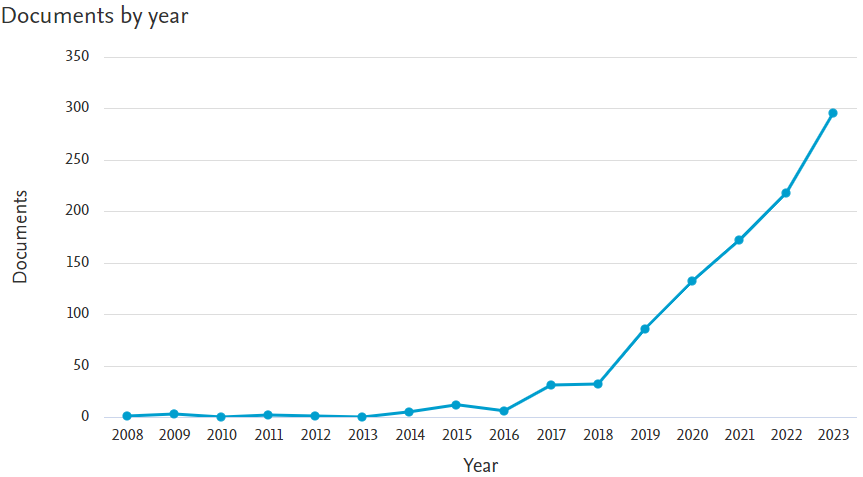
\includegraphics[width=1\textwidth]{Plantilla_TFG_latex//imagenes//Inf//EdA/scopus_mh.png}}
  \hfill
  \subfloat{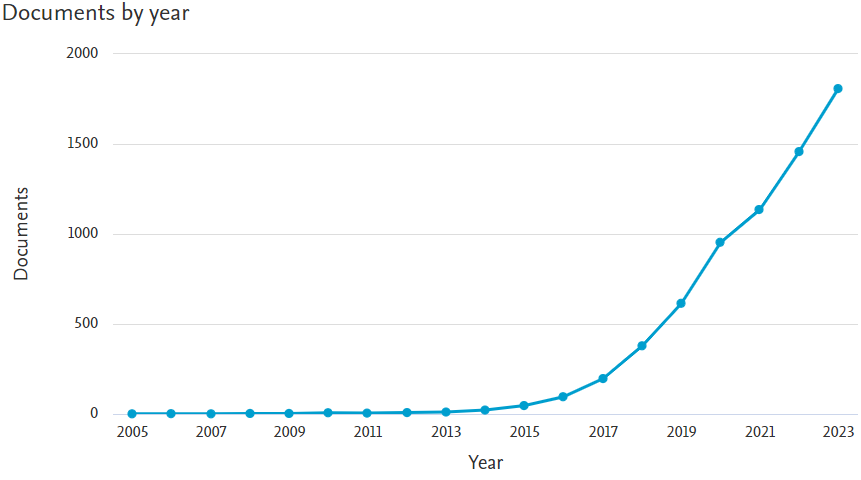
\includegraphics[width=1\textwidth]{Plantilla_TFG_latex//imagenes//Inf//EdA/scopus_gd.png}}
  \caption[Número de documentos indexados anualmente en la base de datos Scopus relacionados con el entrenamiento de modelos de aprendizaje profundo mediante diferentes enfoques]{Número de documentos indexados anualmente en la base de datos Scopus relacionados con el entrenamiento de modelos de aprendizaje profundo mediante diferentes enfoques. La primera gráfica (arriba) muestra la cantidad de artículos que exploran el uso de MH para la optimización del entrenamiento de redes neuronales profundas, obteniendo un total de 997 publicaciones. La segunda gráfica (abajo) presenta el volumen de publicaciones centradas en el entrenamiento basado en GD, obteniendo un total de 6,753, lo que resulta en una diferencia de 7 veces mayor. Se observa que, si bien ambos enfoques han ganado interés en los últimos años, el uso de GD domina ampliamente la producción científica, con un crecimiento exponencial en el número de publicaciones desde 2017. La búsqueda se realiza a fecha del 11 de noviembre de 2024.}
  \label{fig:resEdA}
\end{figure}

Obtenemos una cantidad de 6,753 artículos en lo referente al entrenamiento de modelos de aprendizaje profundo con técnicas basadas en GD y 997 para técnicas MH. \textbf{Vemos que la diferencia entre ambas cantidades es considerable, siendo la primera 7 veces mayor que la segunda}. Destacamos sin embargo que la tendencia en ambos casos es muy similar, como se observa en la Figura \ref{fig:resEdA}, aumentando prácticamente en la misma proporción desde el año 2012.



\subsection{Gradiente descendente y optimizadores}

\textbf{El GD es el algoritmo de aprendizaje utilizado por defecto en prácticamente todas las tareas de aprendizaje profundo, gracias a su eficiencia y buenos resultados}. Los problemas que surgen en su convergencia se intentan evitar en la práctica mediante el desarrollo de modificaciones a su algoritmo, denominadas optimizadores. La literatura en este ámbito es extensa, con una gran variedad de ellos disponibles. A continuación, realizaremos una distinción clara entre optimizadores de primer y de segundo orden.


Aunque los optimizadores de segundo orden presentan mejores propiedades teóricas y ofrecen una convergencia más rápida y estable al utilizar más información del problema, el cálculo o la aproximación de la matriz Hessiana incrementa significativamente el poder computacional necesario para su uso, lo que ralentiza el entrenamiento. Además, hay un problema de memoria: para una red neuronal con 1 millón de parámetros, se requeriría almacenar una matriz de tamaño $1,000,000 \times 1,000,000$, que ocuparía aproximadamente 3,725 GB de memoria RAM. Esto resulta inviable, especialmente considerando que en el top-10 de modelos de clasificación de la competición \textit{ImageNet}, ningún modelo tiene menos de mil millones de parámetros.

Incluso si eliminamos estos inconvenientes de memoria con métodos como L-BFGS (ver Sección \ref{sec:l-bfgs}), enfrentamos un problema significativo: estos métodos requieren el cálculo del gradiente sobre todos los datos de entrenamiento. Conjuntos como \textit{ImageNet}, que contienen más de un millón de ejemplos, hacen que esto sea computacionalmente inviable. Conseguir que este tipo de algoritmos como L-BFGS funcionen con \textit{batches} es más complejo que en MBGD y de hecho es un área abierta de investigación.

En la práctica no es común ver el algoritmo L-BFGS u otros optimizadores de segundo orden aplicados a modelos de aprendizaje profundo a gran escala. En su lugar se utilizan variantes de MBGD basadas en el uso de momento y en tasas de aprendizaje adaptativas, ya que son mucho más simples y más escalables. Existen varias opciones bastante asentadas, que forman parte de las librerías de aprendizaje automático más usadas como PyTorch y TensorFlow, entre las cuales destacan Adam, NAG, RMSProp, AdaGrad o SGD con momento. Vamos a analizar la comparativa \cite{Kyrillidis2020} entre los optimizadores basados en GD con rendimiento del estado del arte para obtener una visión general.

En ella se diferencia entre los algoritmos que tienen tasa de aprendizaje adaptativa (Adam, AMSGrad, AdamW, QHAdam, Demon Adam, YellowFin) y los que no (SGDM, AggMo, QHM, Demon Momentum). Una consideración muy importante que se realiza en dicha comparativa, y que es bien sabida en el campo del aprendizaje automático, es que el rendimiento de una técnica de entrenamiento está muy ligado al dominio específico del problema. Puede ocurrir que un método que no sea de los mejores en términos generales sí lo sea en un problema específico. Pasamos ahora a describir rápidamente las técnicas más interesantes.


YellowFin \cite{yellowfin} es un optimizador con tasa de aprendizaje y momento adaptativos, de manera que mantiene dichos hiperparámetros en un intervalo donde el ratio de convergencia es una constante igual a la raíz del momento. AdamW es una extensión de Adam en la que se utiliza penalización en los pesos del modelo de manera que exista un sesgo hacia valores más pequeños de los mismos durante el entrenamiento, ya que normalmente se asocian valores grandes en los parámetros con el sobreajuste. Aunque Adam ya incorpora este mecanismo, AdamW realiza una pequeña modificación a través de desacoplar esta penalización de la actualización del gradiente, resultando en un impacto notable. 

QHM es una extensión del método de momento clásico que introduce un término cuasi-hiperbólico. Esto permite una mezcla controlada entre el momento y el algoritmo de GD original, proporcionando una mayor flexibilidad y mejorando la estabilidad del entrenamiento. QHAdam combina las ventajas del optimizador Adam con las del GD con momento cuasi-hiperbólico. Introduce factores de amortiguación para controlar la contribución de las medias móviles de primer y segundo orden, ofreciendo un equilibrio entre estabilidad y rapidez en la convergencia. 

Demon Adam es una variante de Adam que ajusta dinámicamente el momento durante el entrenamiento. Utiliza una estrategia de decaimiento del momento para mejorar la adaptación a diferentes fases del entrenamiento, permitiendo una mejor convergencia y evitando caer en mínimos locales. Similar a Demon Adam, Demon Momentum aplica la técnica de decaimiento del momento, pero se usa con optimizadores basados solo en el momento clásico, no en Adam. Mejora la capacidad de adaptación del optimizador durante el entrenamiento al ajustar el momento de manera dinámica. AggMo combina múltiples trayectorias de momento con diferentes factores de decaimiento. Esto ayuda a mejorar la exploración del espacio de parámetros y a mitigar la dependencia de los hiperparámetros del momento, proporcionando una convergencia más robusta y rápida.


Como conclusión, y atendiendo siempre al dominio específico del problema, se establece que YellowFin es la mejor opción en caso de no disponer de recursos para ajustar los hiperparámetros, ya que adapta el momento y la tasa de aprendizaje a lo largo del entrenamiento. Si se dispone de recursos, pero no demasiados, lo mejor son algoritmos de tasa de aprendizaje adaptativa de manera que sólo se tenga que ajustar el valor del momento; en concreto destacan AdamW, QHAdam y Demon Adam. En cambio si se quiere obtener el mejor rendimiento a toda costa, invirtiendo muchos recursos en el ajuste de parámetros, usar MBGD con momento es la mejor opción, aunque sea un método más clásico.


\subsection{Metaheurísticas en el entrenamiento de modelos}

Aún con el uso de optimizadores, hay ciertos inconvenientes en el entrenamiento que son insalvables, como los que están provocados por los cálculos del gradiente con el algoritmo de \textit{backpropagation}. Las técnicas MH son una gran alternativa, ya que sus operadores de búsqueda no dependen de \textit{backpropagation}, evitando así sus problemas. 

Uno de los enfoques de aplicación de estas técnicas es la combinación con las técnicas clásicas, utilizando diferentes aproximaciones. Por ejemplo en \cite{162} se usa el algoritmo \textit{Artificial Bee Colony} \cite{beesalgo} sobre un conjunto de soluciones aleatorias para generar una población inicial de conjuntos de parámetros de un modelo que se entrenan con GD. En \cite{155} se combina un algoritmo genético con el GD, de manera que las nuevas soluciones son generadas con el operador de búsqueda del primero pero son evaluadas tras realizar varias épocas con el segundo. De manera similar en \cite{163} se usa la técnica MH \textit{Particle Swarm Optimization} \cite{pso} para entrenar los parámetros de la última capa de una ConvNet, mientras que el resto se entrenan a través del algoritmo de GD. La comparación arroja que la hibridación de ambas técnicas alcanza mejores resultados en términos de rapidez de convergencia y de \textit{accuracy}. Prácticamente la totalidad de la literatura referente a esta estrategia está centrada en ConvNets.

Otro enfoque es entrenar el modelo usando exclusivamente algoritmos MH. En este ámbito destacan los estudios \cite{174} y \cite{176}, en los que se proponen dos técnicas basadas en \textit{Simulated Annealing} \cite{siman} para entrenar los parámetros de una ConvNet, consiguiendo mejor rendimiento y mayor velocidad de convergencia que en el mismo modelo entrenado mediante el algoritmo de GD. Al igual que ocurre con el enfoque anterior, la gran mayoría de estos estudios están centrados en ConvNets y \textit{Recurrent Neural Networks}. 

Algo importante a destacar en la literatura de entrenamiento de modelos con técnicas MH es la falta de un marco común en los estudios, lo que impide realizar comparaciones objetivas entre ellos. Esta cuestión, comentada con más detalle en la Sección \ref{sec:motinfo}, evidencia la necesidad de más experimentos bajo condiciones similares para poder sacar conclusiones objetivas entre ellos.

\textbf{El rendimiento de estas técnicas todavía no es comparable al de las técnicas clásicas. Si bien es cierto que para tareas sencillas y modelos con pocos parámetros pueden mejorar al GD en la minimización de la función de pérdida, generalmente en términos de generalización su rendimiento es inferior. Además, es importante considerar la complejidad computacional: para alcanzar un rendimiento similar al del GD, estas técnicas requieren mucho más tiempo y recursos computacionales, por lo que no resultan una alternativa viable para este tipo de tareas.}






\subsection{Neuroevolución}

La neuroevolución es un enfoque que combina algoritmos evolutivos con redes neuronales, con el objetivo de optimizar sus pesos, arquitecturas o reglas de aprendizaje \cite{Yao1999}. A diferencia de los métodos de optimización basados en gradiente, la neuroevolución utiliza principios inspirados en la evolución biológica para desarrollar y entrenar redes neuronales, ofreciendo alternativas robustas especialmente en escenarios donde el cálculo de gradientes resulta complejo o inviable.



El paradigma de la neuroevolución se basa en la aplicación de operadores evolutivos (selección, cruce y mutación) para desarrollar redes neuronales, sin depender de información de gradiente. \cite{Whitley1990} establecieron algunas de las bases iniciales al demostrar cómo los algoritmos genéticos podían optimizar tanto las conexiones como la conectividad en redes neuronales. Este enfoque resulta particularmente valioso en problemas con espacios de búsqueda no diferenciables, funciones objetivo ruidosas o con múltiples óptimos locales \cite{Stanley2019}. La neuroevolución puede aplicarse a diferentes aspectos de las redes neuronales:

\begin{itemize}
    \item Optimización de pesos: evolucionamos los parámetros del modelo.
    \item Evolución de arquitecturas: donde la topología de la red (número de capas, neuronas y conexiones) es determinada evolutivamente.
    \item Evolución de reglas de aprendizaje: donde los propios algoritmos de aprendizaje son evolucionados.
\end{itemize}




El algoritmo \textit{NeuroEvolution of Augmenting Topologies} (NEAT), propuesto por \cite{Stanley2002}, representa uno de los avances más significativos en neuroevolución. NEAT permite la evolución simultánea de la topología y los pesos de las redes neuronales, comenzando con estructuras mínimas que gradualmente se vuelven más complejas. Este enfoque ha demostrado capacidad para generar soluciones más compactas y eficientes que otros métodos neuroevolutivos convencionales. Sus características distintivas incluyen:

\begin{enumerate}
    \item Operadores de mutación que pueden añadir nodos y conexiones.
    \item Un sistema de marcado histórico que resuelve el problema de cruzamiento entre redes con diferentes topologías.
    \item Especiación para asegurar innovaciones estructurales.
\end{enumerate}





Con el auge del aprendizaje profundo, la investigación ha evolucionado hacia la aplicación de técnicas evolutivas en redes neuronales de múltiples capas. \cite{David2014} presentaron un enfoque para evolucionar redes neuronales profundas mediante algoritmos genéticos, demostrando su viabilidad en problemas de clasificación. \cite{Such2017} ampliaron este campo al demostrar que los algoritmos genéticos constituyen una alternativa competitiva frente a métodos como el aprendizaje por refuerzo profundo. Su investigación reveló que la simple búsqueda de mutaciones en el espacio de pesos de redes neuronales puede superar a algoritmos complejos basados en gradiente en ciertas tareas de refuerzo. 



La neuroevolución ha encontrado aplicaciones en diversas áreas:



\begin{enumerate}
    \item \textbf{Aprendizaje por refuerzo}: Donde la ausencia de gradientes claros dificulta los métodos tradicionales. \cite{Miikkulainen2019} demostraron la eficacia de la neuroevolución en entornos de aprendizaje por refuerzo complejos.

    \item \textbf{Redes neuronales de impulsos (\textit{Spiking Neural Networks})}: \cite{Pavlidis2005} aplicaron algoritmos evolutivos para entrenar este tipo de redes, donde los métodos basados en gradiente resultan particularmente difíciles de implementar debido a la naturaleza discontinua de los impulsos neuronales.

    \item \textbf{Problemas con funciones objetivo no diferenciables}: La neuroevolución permite optimizar redes neuronales respecto a criterios que no proporcionan gradientes, como métricas discretas o comportamientos emergentes complejos.
\end{enumerate}


En artículos recientes, \cite{Stanley2019} sugieren que el futuro de la neuroevolución reside en su capacidad para descubrir arquitecturas novedosas y adaptativas, complementando más que compitiendo con los métodos basados en gradiente. Esta visión híbrida podría conducir a sistemas que combinen la eficiencia local del GD con la exploración global de los métodos evolutivos. En \cite{Slowik2008} se demuestra cómo los algoritmos de evolución diferencial pueden complementar los métodos tradicionales de entrenamiento, ofreciendo mejoras significativas en términos de tiempo de convergencia y calidad de las soluciones. La revisión comprehensiva de \cite{Kaveh2023} sobre algoritmos MH para el entrenamiento de redes neuronales confirma esta tendencia hacia enfoques híbridos, donde la neuroevolución juega un papel fundamental en la optimización global del proceso de aprendizaje, mientras que los métodos basados en gradiente se encargan del refinamiento local.



\subsection{Aprendizaje Automático Automatizado}

El Aprendizaje Automático Automatizado (AutoML) emerge como una respuesta a la creciente complejidad y especialización requerida en el desarrollo de modelos de aprendizaje automático. Esta disciplina busca automatizar el proceso de selección, configuración y optimización de modelos, reduciendo la necesidad de intervención humana especializada y democratizando el acceso a técnicas avanzadas de aprendizaje automático \cite{Hutter2019}.

Esta automatización se fundamenta en métodos de búsqueda y optimización que evalúan iterativamente diferentes configuraciones, buscando maximizar métricas de rendimiento definidas \cite{Hutter2019}. La relación entre AutoML y las MH es estrecha, ya que muchas técnicas de AutoML utilizan algoritmos evolutivos, búsqueda bayesiana u otros métodos MH como motores de optimización \cite{Kaveh2023}.

La optimización bayesiana constituye uno de los enfoques más utilizados en AutoML, modelando la función objetivo (el rendimiento del modelo) como un proceso gaussiano y utilizando técnicas de adquisición para seleccionar puntos de evaluación prometedores. Este enfoque permite balancear eficientemente la exploración y explotación en el espacio de hiperparámetros \cite{Shahriari2016}.


Los algoritmos evolutivos ofrecen una alternativa robusta para la optimización en AutoML. En \cite{Alba2006} documentan cómo diversos procedimientos MH, incluyendo algoritmos genéticos y evolución diferencial, pueden aplicarse efectivamente al entrenamiento y configuración de redes neuronales. Estos métodos resultan particularmente valiosos para espacios de búsqueda complejos y no diferenciables.

\cite{Miikkulainen2019} proponen la evolución de redes neuronales profundas completas, incluyendo tanto arquitecturas como hiperparámetros, demostrando que los métodos evolutivos pueden generar soluciones competitivas para problemas complejos de aprendizaje automático.


Los algoritmos de \textit{multi-armed bandit} y sus variantes permiten la asignación dinámica de recursos computacionales a configuraciones prometedoras, descartando eficientemente opciones subóptimas. Estos métodos han sido implementados en sistemas como \textit{Hyperband} \cite{Li2018}, que combina la búsqueda aleatoria con una estrategia de asignación de recursos basada en \textit{bandits}.

Aunque AutoML busca reducir la necesidad de experiencia humana, la integración efectiva de conocimiento experto en el proceso automatizado representa un área de investigación prometedora. Los enfoques que permiten a los expertos guiar el proceso de búsqueda o incorporar restricciones específicas del dominio podrían mejorar significativamente la efectividad de los sistemas AutoML \cite{Hutter2019}. Las direcciones futuras apuntan hacia sistemas más integrados que combinen diferentes enfoques de optimización, aprovechando tanto métodos basados en gradiente como MH evolutivas, y que puedan adaptarse dinámicamente a los requisitos específicos de cada problema \cite{Elsken2019}.












\subsection{Búsqueda de Arquitectura Neuronal}

Búsqueda de Arquitectura Neuronal (NAS, por sus siglas en inglés, \textit{Neural Architecture Seach}) representa un subcampo especializado dentro del AutoML, centrado específicamente en la automatización del diseño de arquitecturas de redes neuronales. Esta disciplina busca sustituir el proceso manual de diseño arquitectónico por metodologías algorítmicas que puedan descubrir estructuras óptimas o casi óptimas para problemas específicos \cite{Elsken2019}. El diseño manual de arquitecturas neuronales ha sido tradicionalmente un proceso que requiere considerable experiencia y conocimiento especializado, además de seguir un ciclo iterativo de prueba y error. Esta complejidad ha motivado el desarrollo de métodos automáticos que puedan explorar sistemáticamente el espacio de arquitecturas posibles \cite{Zoph2017}.


Los métodos de NAS pueden clasificarse en tres grupos: basados en aprendizaje por refuerzo, evolutivos y basados en gradiente. Los primeros formulan el diseño arquitectónico como un problema de decisión secuencial, donde un agente aprende a seleccionar componentes arquitectónicos que maximizan métricas de rendimiento. El trabajo pionero de \cite{Zoph2017} demostró la viabilidad de este enfoque, utilizando redes neuronales recurrentes como controladores para generar descripciones de arquitecturas.

Los algoritmos evolutivos constituyen una alternativa robusta para NAS, al modelar las arquitecturas como individuos dentro de una población que evoluciona mediante operadores genéticos. Un ejemplo destacado de este enfoque es el trabajo de Xie et al., quienes propusieron un método basado en algoritmos genéticos para evolucionar arquitecturas de redes convolucionales, logrando resultados competitivos en tareas de clasificación de imágenes \cite{Xie2017}. Posteriormente, Lu et al. ampliaron este enfoque con NSGA-Net, un algoritmo genético multiobjetivo diseñado para optimizar de manera simultánea la precisión y la complejidad computacional de las arquitecturas \cite{Lu2018}. Este trabajo evidencia cómo los métodos evolutivos pueden abordar de manera eficaz la naturaleza multiobjetivo inherente al diseño de arquitecturas neuronales. Por otro lado, Stanley et al. destacan las ventajas de la neuroevolución en el contexto de NAS, subrayando su capacidad para explorar de forma eficiente espacios de búsqueda complejos y no diferenciables \cite{Stanley2019}. En esta línea, el algoritmo NEAT, desarrollado por Stanley y Miikkulainen, ofrece un marco natural para la evolución de topologías neuronales, lo que lo convierte en una estrategia adecuada para la búsqueda automatizada de arquitecturas \cite{Stanley2002}.




A diferencia de los enfoques anteriores, los métodos basados en gradiente relajan el problema discreto de selección arquitectónica a un problema continuo, permitiendo la aplicación de técnicas de optimización basadas en gradiente. DARTS (\textit{Differentiable Architecture Search}) ejemplifica este enfoque, utilizando relajaciones \textit{softmax} para hacer diferenciable el proceso de selección de operaciones \cite{Liu2018}.



La principal limitación de NAS es su coste computacional, lo que ha motivado diversas estrategias para mejorar su eficiencia, como compartir pesos entre las distintas arquitecturas candidatas \cite{Pham2018} en ENAS (\textit{Efficient Neural Architecture Search}), usar tareas simplificadas o predictores de rendimiento para ahorrar coste computacional \cite{Baker2018}, o descomposición jerárquica del problema en otros más pequeños (entrenar partes de la arquitectura por separado y luego combinarlas) \cite{Miikkulainen2019,Liu2018}.


Los estudios comparativos entre arquitecturas generadas automáticamente y diseñadas manualmente han arrojado resultados significativos:

\begin{enumerate}
\item \textbf{Rendimiento}: En diversas tareas, las arquitecturas generadas mediante NAS han igualado o superado a las diseñadas manualmente. Por ejemplo, NASNet \cite{Zoph2018} superó el rendimiento de ResNet e Inception en tareas de clasificación de imágenes.

\item \textbf{Eficiencia computacional}: Mediante optimización multiobjetivo, como en NSGA-Net \cite{Lu2018}, es posible generar arquitecturas que balancean precisión y eficiencia computacional, superando a modelos manuales en ambas dimensiones.

\item \textbf{Transferibilidad}: Las arquitecturas descubiertas en tareas específicas han demostrado buena capacidad de transferencia a otras tareas relacionadas, sugiriendo que NAS puede identificar estructuras con propiedades generalizables \cite{Lu2018}.

\item \textbf{Novedad estructural}: Los métodos de NAS han descubierto estructuras novedosas que difieren significativamente de los diseños convencionales, como conexiones densas no intuitivas o patrones de conexión irregulares \cite{Real2019}.
\end{enumerate}



La adaptación de NAS a dominios específicos como redes neuronales recurrentes, redes generativas adversarias o redes de grafos representa un área de investigación activa \cite{Gao2020}. La integración de NAS con otros componentes del ciclo de aprendizaje automático, como la selección de características o la optimización de hiperparámetros, apunta hacia sistemas más comprensivos que puedan optimizar \textit{pipelines} completos de aprendizaje automático \cite{Kaveh2023}. La evolución de NAS refleja una tendencia más amplia hacia la automatización del diseño de sistemas de aprendizaje automático, donde los métodos evolutivos y otras MH juegan un papel fundamental al proporcionar marcos robustos para la exploración de espacios de diseño complejos y no diferenciables.




